
% .
% \newpage
% \newpage
 
 \changefont{ppl}{m}{n}
 
  %\maketitle
   
 \begin{titlepage} 

%\includegraphics[width=0.9\textwidth]{/home/felicitas/133_1.JPG}

\begin{pspicture}
(-4.9,8.5)
\rput(0cm,0cm){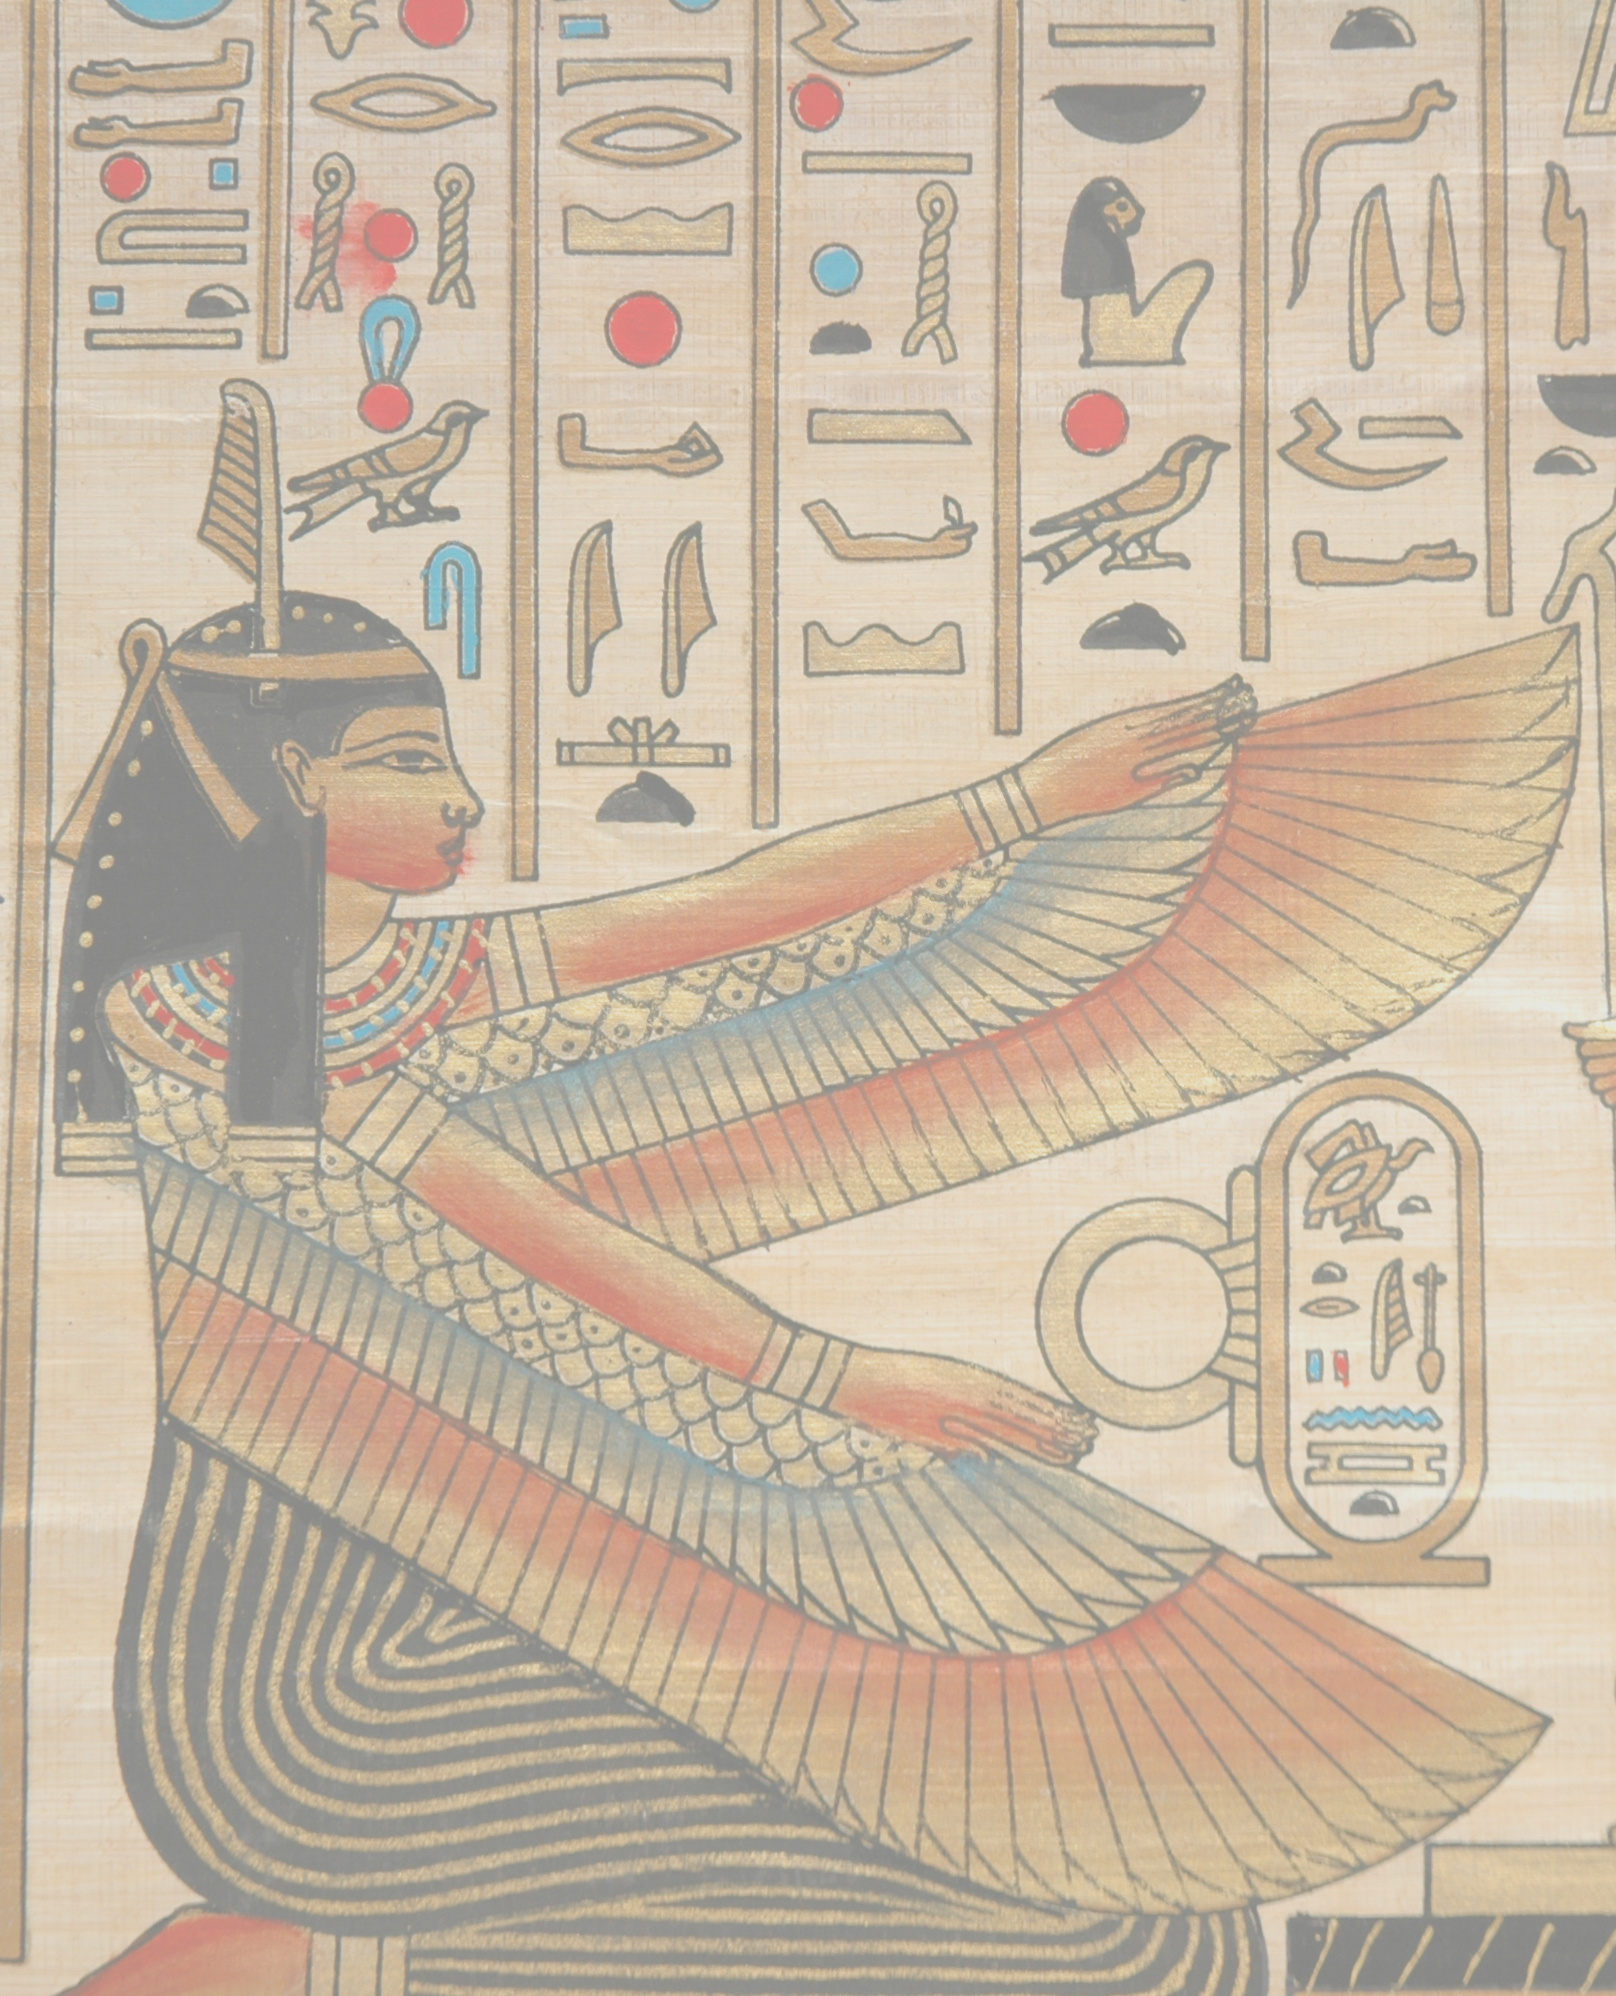
\includegraphics[width=\paperwidth,height=\paperheight]{Titel-Hell}}
\end{pspicture}
  
  \vspace*{-0.4\textheight}
  {\fontsize{40}{60}\selectfont Die Horussöhne}\\[38ex]
  {\huge Felicitas Stotz}\\[8ex]
   \today
 
 \end{titlepage}


\thispagestyle{empty}


\chapter*{}

\section*{Titelei}

%\begin{tg}
\begin{verse}



Die Schrift des Verborgenen Raumes.\\
Die Standorte der Bau und der Götter,\\
die Schatten und Achu, und was getan wird.

Der Anfang ist das Horn des Westens,\\
das Tor des Westhorizontes;\\
das Ende ist die Urfinsternis,\\
das Tor des Westhorizontes.

Zu kennen die Unterweltlichen Bau,\\
zu kennen die Geheimen Bau,\\
zu kennen die Tore\\
und die Wege, auf denen der Grösste Gott wandelt.

Zu kennen, was getan wird, \\
zu kennen, was in den Stunden ist, und ihre Götter, \\
zu kennen den Lauf der Stunden, und ihre Götter.


Zu kennen ihre Verklärungen des RE,\\
zu kennen, was er ihnen zuruft,\\
zu kennen die Gedeihenden und die Ver\-nich\-te\-ten.{}\\

\end{verse}
%\end{tg}



\chapter*{2. Februar (Prolog)}
\addcontentsline{toc}{chapter}{Prolog: 2 . Februar (Prolog)}

Die Wahrheit ist: Wir wissen es nicht! 

Was wir wissen, sind die Dinge, die wir wahr-nehmen. Wir nehmen sie mit unseren Sinnen auf und bewerten sie. Dabei bewerten wir sie nach nützlich oder unnütz, essbar oder nicht essbar und kommt es für die Paarung in Frage? Wenn wir die Dinge als wahr bezeichnen, die wir mit den Sinnen in der physischen Welt erfahren, sind wir auf der sichereren Seite. Nicht ganz sicher, aber immerhin\dots

Dann gibt es unser Gehirn, unsere Emotionen, unsere Träume, unsere Hoffnungen und Wünsche, unsere Ängste, unseren Glauben\dots Sie sind unsichtbar, unfassbar, aber denkbar. Das ist interessant, weil wir in unserem Gehirn die sichtbaren Wahrnehmungen und die unsichtbaren Gedanken miteinander untrennbar vermischen. Und weil wir sie vermischen, wissen wir schliesslich nicht mehr, was wir wahrnehmen könnten und was denken. Wissen wir nicht, was wir erfahren haben, was wir kennen und was wir nicht wissen können, weil wir es mit einem grauen, weichen Fleischklops gedacht haben.

Wir neigen dazu, uns für alles eine Antwort zu basteln. Denn eine erklärbare Welt ist eine überschaubare Welt. Eine Welt, in der man weiss, wo der Tiger wohnt\dots \footnote{Eine beliebte Tiger-Adresse ist der indische Dschungel und Sibirien.} Dann kommen wir mit den Unsichtbarkeiten unseres Daseins besser zurecht. Den dunklen Gedanken in der Nacht, wenn wir nicht mehr sicher sind, ob wir wissen, wo der Tiger wohnt.

Und wenn wir die samtweichen Tigerpranken an unserem Schlafpelz vorbei schleichen hören, wünschen wir uns jemanden, der uns beschützt. Einen Krieger! Zwei starke Krieger! Zwanzig starke Krieger!

 Viele, starke Riesenkrieger, die dem Tiger in den Hinter treten und ihn im hohen Bogen bis nach Sibirien schicken, damit wir genau wissen, wo er wohnt und sich seinen  verd***ten, schmerzenden, kalten Hintern schleckt! Weit weg im verd***t Sibirien!
 
Vielleicht, -wir wissen es nicht. Vielleicht sind so die ersten Götter entstanden? => Götter = Tigerschnelllieferservice für die Russen! 

Und wenn wir beginnen unser Gehirn für Erklärungen der Dinge zu bemühen, die wir nicht verstehen, dann könnten wir auf die Idee kommen, der Tigerschnelllieferservice könnte viel mehr.

Vielleicht würden wir die Chance ergreifen und uns vorstellen, dass die starken Riesenkrieger die Welt erschaffen haben. Und wenn sie zusammen schaffen, dann brauchen sie einen Chef! Und wo wohnt der Chef der starken Riesenkrieger, während seine Jungs die Welt bauen? Logisch, auf der Sonne! Die ist ein würdiger Chefsessel! Und wo starke Jungs sind und ein Chef, da dürfen auch die Frauen und Mütter nicht fehlen\dots 

Et voila! Fertig ist die Götterwelt! Gibt es sie, gibt es sie nicht? Wir wissen es nicht. Was wir jedoch wissen und kennen, ist die Sehnsucht die Dinge zu verstehen, die Fäden der Geschichte zu finden, damit wir etwas haben, an dem wir unseren Sinn finden und ihm folgen können. Götter können dafür ein nützliches Konzept bereit halten. Eine gute Erklärung, wieso es die Welt gibt und eine, die die Verantwortlichkeiten klärt.

=> Götter = Weltenerbauer => Verantwortlich = Praktisch\footnote{Sich im Geiste Dinge vorzustellen um Informationen zu bekommen, ist völlig okay. Schliesslich haben wir diese tolle Denkkiste in unserem Kopf. Schwierigkeiten bekommen wir dann, wenn wir uns von unserem exzentrischen Denkkasten Unsichtbarkeiten als Dogmen verkaufen lassen! Also, wenn ein kleiner, grüner Zwerg Dir sagt, was Du tun sollst, dann hör nicht auf ihn. Wenn er Dir jedoch interessante Informationen zukommen lässt, dann brauche sie bei Deiner Entscheidungssuche. Allerdings erst, wenn Du darüber nachgedacht hast.}

Götter sind kreativ und eine ihre beliebtesten Hauptaufgaben ist die Schöpfung. Es gibt viele verschiedene Versionen und Ideen bei den Menschen, wie die Erde in den Zustand gekommen ist, in dem sie sich zur Zeit befindet. Und viele Jahrtausende waren sich unsere Vorfahren einig, es sind Götter gewesen. Einer, viele, egal, aber Götter. Unsichtbare, dem Menschen überlegene Wesen, die alles mehr oder weniger leiteten und im Griff hatten.

Heute, nur am Rande bemerkt, lachen die Menschen über dieses Konzept. Sie glauben nicht an Götter, sondern an die Wissenschaft, was bedeutet, alles hat sich entwickelt. Wie genau das gegangen ist, ist so kompliziert, das verstehen nur wenige. (Früher nannte man die Wenigen mit dem "`geheimen Wissen"' "`Eingeweihte"' und dieses Wissen wurde eifersüchtig von ihnen gehütet, aber das war früher. Ha! Hahaha! Heute nennt man es Lizenzrecht.) 

Wenn wir verschiedene Schöpfungsgeschichten anschauen, werden wir feststellen, Götter sind nicht nett. Und in diesem Sinne, liegt auch in unserer Zeit die Frage nahe, ob der Mensch nicht doch göttlichen Ursprunges ist.\footnote{Das liegt näher, als die Vermutung, einiger heutiger "`Eingeweihter"', die glauben, der Mensch sei ein Affe. Aber die Affen können nichts für den Zustand der Erde und es ist gemein, sie ungefragt in die Sache mit der Erde und den menschlichen Zerstörungsversuchen mit hinein zu ziehen. Das haben sie nicht verdient, für ihre Ähnlichkeit mit den Menschen können sie schliesslich nichts.}

\sterne

Unsere Geschichte einer göttlichen Reisegruppe beginnt an einer Stelle der Schöpfung, als die Menschheit sich an einem ähnlichen Punkt befand wie wir heute, wenn wir alten Überlieferungen glauben. Natürlich war dennoch alles anders\dots

Nebelverhangen war das Land Atlantis. Die Menschen besassen weder einen Körper, wie wir ihn kennen, noch hatten sie unser heutiges Bewusstsein. Die Menschen, sie träumten, auch wenn sie wach waren. Dabei waren die Atlantier hoch begabt: Sie waren hellsichtig und konnten die Kräfte, die in den Pflanzen und Steinen vorhanden waren auf diese Weise nutzten.  Sie flogen in Fahrzeugen herum, die mit der Kraft ihrer Gedanken und Kristallen angetrieben waren.

Während wir uns dies schwer vorstellen können, hätten die Atlantier vielleicht unsere Form der Fortbewegung überraschen gefunden: Wir nutzen die Kräfte der Natur, dank unserer weit entwickelten Fähigkeit zu denken. Damit haben wir ein Gefährt entwickelt, das aus Metall gebaut ist und mit Pflanzenkraft angetrieben wird, das Auto.

Was die Atlantier jedoch am meisten von uns heute unterschied, ist nicht ihr merkwürdiger zu Beginn dieser Zeit knochenloser Körper und ihre Hellsichtigkeit, die ihnen ein ähnlich komfortables, weitentwickeltes Leben bescherte. Nein, der grösste Unterschied war, sie kannten ihre Götter! Persönlich. Mit Vor- und Nachnamen und Adresse! Was nicht viel half, denn wie wir wissen, ging Atlantis kläglich unter.

Einer, der nicht unterging, so sagt es die Legende, weil er weise war und sich deshalb dem Wohlwollen der atlantischen Götter erfreute, war Thot. Thot konnte vor dem Untergang von Atlantis flüchten. Und der damals sehr begabte, aber menschliche Thot floh nach Ägypten und fand dort für sich und sein geheimes, atlantisches Wissen eine neue Heimat.

Thot wurde später selbst Gott im Ägypten und war auch bei den Griechen kein unbekannter. Im Gegenteil, sie nannten ihn, wiederum nach ihrem Gott Hermes: Hermes Trismegistos. Thot war ein Tüftler, Erfinder und Philosoph. Dabei ist er nicht der mächtigste der ägyptischen Götter\dots


Er ist allerdings der Gott, der sich am besten als Reiseleiter eignet, weil er selbst als Mensch seine Karriere begonnen hat. Für eine Reisegruppe von Göttern, die teilweise nicht über menschliche Körper verfügen, oder nie aus dem Jenseits, das in Ägypten Duat heisst, heraus gekommen sind, ist es von Vorteil einen gut informierten Reiseleiter zu haben.

Der Jenseitsbereich ist um die Erde herum, ein riesiger Raum für alle Götter, die für die Erde zuständig sind und die Verstorbenen. Allerdings haben die Götter des einen Zeitalters, des einen oder anderen Landes ihre ganz spezifischen Aufgaben. Nicht alle Götter kümmern sich um alles. Andere haben sich auf den "`Altenteil"' zurückgezogen und geben den jüngeren Göttern Tipps, wie man tüchtige Blitze schleudern kann, ohne dabei die ganze Gemeinde auszulöschen. Im Laufe der Zeit hat sich dieser Bereich genauso weiterentwickelt wie die Erde und Menschen.

Wenn Menschen jedoch einen unbestechlichen Wächtergott auf grausame Weise hintergehen, seinen Schutzbefohlenen schaden und damit seine Unbestechlickeit ins Wanken bringen, wenn ein Gott, der in Rente gegangen ist, leiden muss, weil er seiner Zeit voraus war, und er jetzt die Chance der Heilung hat und wenn eine uralte Göttin nicht einmal als Hausmädchen getarnt, ihre geheimen Initiationen durchführen kann, weil plötzlich ein Fluch auftaucht, dann können auch alte Götter sich für eine Reise entschliessen und internationale zusammenarbeiten..

Und so kommt es, dass der grosse Hermes Trismegistos, der "`dreimal grosse Hermes"' genannte Thot, in einer kalten, nebeligen Nacht nach Basel kommt. Er war verabredet und wollte gleichzeitig eine Unterkunft für seine Reisegruppe in Augenschein nehmen.

Thot kannte seine Pappenheimer an jedem Ort. Ihm blieb kein Ort an dem hermetische Künste eine Rolle spielten unbekannt. In Basel einen Wohnort für sein buntes Reisegrüppchen zu finden war einfach. Was liegt näher als die Damen und Herren an dem Ort unterzubringen, an dem ein ehemaliger Adept der Alchemie und Hermetik seinen grossen Auftritt hatte: der grosse Cagliostro? Für die einen ein Scharlatan und für die anderen ein Grossmeister der ägyptischen Logen und Besitzer des Steines der Weisen. Als Thot am Rheinsprung vor den zwei grossen Häusern der Gebrüder Sarasin stand, nickte er zufrieden. Schliesslich wollen auch die abenteuerlustigsten Götter und vor allem Göttinnen nicht auf einen Hauch an Luxus verzichten.

Im berühmten Oktagon, dem achteckigen Zimmer des weissen Hauses des ehrwürdigen Jakob Sarasin, trifft sich der alte ägyptische Gott mit seinen nordischen Freunden Berta, auch bekannt als Frau Holle und Hans, dem "`Wilde Maa"'.

Während Thot sich in einen Ohrensessel gesetzt hatte, von denen zwei im Raum standen, lief Berta im Raum auf und ab. Sie steckte in einem langen schwarzen Kleid und einer weissen Schürze. Sie sah aus wie ein altes, verhutzeltes Hausmädchen. In ihren grauen, kurzen Locken steckt ein weisses Häubchen. Ab und zu schauten ihre Füsse, die in derben, braunen, orthopädischen Schuhen stecken unter dem Kleid hervor. Vor der Tür im Gang stand ein Reisigbesen. Ab und zu nahm sie einen Schluck aus dem Kristallglas, das mit einem rauchig duftenden, bernsteinfarbenem Whisky gefüllt war. Es stand auf einem kleinen runden Nussholztischchen.

Ein zartes Grunzen ertönte. Von dem zierlichen, mit Seide bezogenem Sofa, schauten nur die geschwungenen, dünnen Beinchen hervor, der Rest war unter  dem wilden Mann begraben. Ausser einem Schurz aus Laub, Fell und Zweigen und einer Krone aus Eichenlaub war er nackt. Seine Haut schimmerte goldbraun und unter der Haut zeichneten sich die kräftigen Muskeln ab. Das Gesicht war faltig und die wilden Locken schimmerten nicht nur braun und rot, sondern grün. Da das Sofa viel zu klein war, hing ein Bein über die Lehne und das andere ragte weit ins Zimmer. Eine Hand lag auf den Boden und wenn der Wilde Mann schnarchte, zitterten die Blätter seiner Krone hingebungsvoll. Vor dem Sofa lag ein Dackel. Er hatte sich lang ausgestreckt und sah aus wie eine Pelzwurst mit vier kurzen Beinen und einer schwarzen Nase. Der Dackel schnarchte mit seinem Herrchen in bachscher Fugenmanier. Draussen hörten Berta und Thot einige Krähen von den Dächern krächzen.
 
"`Interessant, äusserst interessant!"' Thot legte die schlanken Fingerspitzen aneinander. Er bevorzugte einen zeitgenössischen, schlichten, schwarzen Anzug. Sein Hemd war weiss-grau gestreift und er trug eine hellgraue Krawatte. In einer angesehenen Anwaltskanzlei wäre er heutigen Tages vermutlich nicht aufgefallen. Er hatte eine schmale, aber lange Nase. Die hellblauen, kristallklaren Augen, lagen tief und waren von der Stirn und den Augenbrauen verborgen. Seine schwarzen Haare lagen wie ein lockiger Helm um seinen Kopf und waren mit grauen Strähnen durchzogen. 

Er hatte die langen, schlanken Beine übereinander geschlagen und wippte unrhythmisch mit dem Fuss. "`Und was schliesst du daraus, verehrte Berta?"' "`Lieber Thot, wenn ich es selber wüsste, hätte ich Euch wohl kaum hierher bemüht!"' sagte Berta und liess ratlos die Arme fallen. Thot sagte entschieden: "`Im Moment werde ich gerne bemüht. Mir ist langweilig geworden im Jenseits und den anderen Herrschaften auch. Wir können Bewegung brauchen, sowohl für den Kopf, als auch für die Beine!"' "`Ich bin sicher, da kann ich dir helfen, Thot. Da ist etwas ganz finsteres im Gange, das hab ich in den Knochen."' 

Berta wendete sich dem mannhaften Laubhaufen auf dem Sofa zu: "`Hans? Hans, was sagst Du dazu?"' "`Wckl? Was?"' es dauerte einige Zeit bis sich der Halbgott sortiert hatte und sich aufsetzte. Er stöhnte, schnaufte und hielt sich den Kopf. Berta betrachtete das Spektakel, die Hände auf die breiten Hüften gestemmt:  "`Herrjeh, dann hat er einmal im Jahr seinen grossen Auftritt und danach ist er Wochenlang nicht zu brauchen! Dir tut etwas mehr Bewegung gut, alter Mann!"' rief sie und fuchtelte Hans mit dem kleinen, dicken Zeigefinger vor der Nase herum. Er ächzte: "`Alter Mann?! Also nai, Berta, eso nit!"' Er richtete sich zu seiner vollen Grösse auf und sah der kleinen, kugeligen Frau Holle, die feixend vor ihm stand, sitzend direkt in die Augen.

 "`Fein, dann ist es beschlossen?"' Thot schmunzelte, sie waren sich überall ähnlich, die alten Herrschaften \dots Vergnügt nahm er Stück von der feinen Mandelschokolade, die auf einem feinen Porzellanteller für ihn auf dem Tisch stand. 

"`Wo? Ich persönlich würde Basel vorziehen, da ich selbst etwas erledigen will, was in Ägypten nicht möglich ist!"' murmelte Thot mit einem Rest Schokolade im Mund. "`Hans? Was meinst Du?"' Berta, die einen kräftigen Schluck aus ihrem Glas genommen hatte, wendete sich an Hans. "`Basel!"' sagte Hans. 

Er nahm sich das Bierglas, das neben dem Sofa auf dem Boden gestanden und nun eine Schaumkrone auf dem wertvollen Perserteppich hinterlassen hatte: "`Mr mache s in Basel!"' Er schleckte sich mit der Zunge den Schaum von den Lippen und schaute die anderen beiden versonnen an: "`D Basler sind frommi Leut aber heuer hent sie mit sich und ihre Gschäft z tue. Sie sind gnueg igbildt, ihne werde me oder wenigr Göttr hier nit uffalle. Und z Basel und Umgäbig hätts viili Lütt, wo dr Thot kenne und wo ich kenn, und dir, Berta, lieg jo s Dreiländreck e z Füesse."' Berta warf einen tiefen Blick in ihr Whiskyglas: "`Gut, klingt vernünftig, auch, wenn es von dir kommt!"' "`Berta! Eso, würkli nit!"' meinte Hans freundlich.   

"`Das Wann dürfte allen klar sein?"' fragte Berta. "`Berta!"' rief Hans genervt "`mr sind do keini Deppe!"' "`Natürlich, liebe Berta!"' Thot erhob sich und streckte die langen Glieder. Er war zwar nicht so muskulös wie Hans, aber genauso gross.

"`Ja dann, see you later mit alligator\dots"' Hans lachte grollend.  Berta hatte unter den vielen Falten ihres Kleides gewühlt und nach einiger Zeit Handschuhe zum Vorschein gebracht ("`Dort bleiben sie schön warm!"' hatte sie dem schaudernden Thot augenzwinkernd erklärt). Sie schwang sich auf den Besen und streifte die Handschuhe über.  Hans packte die Göttinnenkugel und stellte sie auf das Sims des geöffneten Fensters:"`Bis Mitwinter!"' rief sie und verschwand im Nebel. "`Es sind Krokodile!"' sagte Thot: "`Keine Alligatoren, sondern Krokodile. Bis Heilig Abend."'

\section*{23. Dezember}
\addcontentsline{toc}{section}{23. Dezember}

"`Hermes, min Fründ, d Berta macht jetzt alles parat für de Transport. Sind dr do z Basel au parat?"' "`Wir sind bereit, Hans. Die Koffer sind gepackt."' antwortete Thot. Er schmunzelte, Hans war sein europäischer Name 'Hermes' offenbar lieber. "`Is' d Alessandro fertig mitmm Schutznetz? Hät er de Zeitüberschneidung richtig usgrechnet?"' "`Ja, ich habe es überprüft. Und unser Alessandro, Graf von Cagliostro, ist ein wahrer Spezialist, wenn es darum geht einen Ort in zwei Zeitzonen einzuteilen. Schliesslich ist diese Fähigkeit sehr nützlich, wenn man, wie er, gerne dem schönen Geschlecht huldigt."' "`Ei, das hesch schön gesagt, dem 'schönen Geschlecht' huldigen\dots So isses, Hermes, d Herr Graf isch kein Kind vo Traurigkeit, des isch woor!"' 

"`Die Häuser werden in der Gegenwart am Tag benutzt, dort befindet sich ein Departement der Stadtregierung. In den Tagen der Rauhnächte werden weniger Menschen dort sein. Sie stören uns nicht und sehen können sie uns auch nicht. Der eine oder andere Mensch wird Kopfschmerzen haben und wirre Träume, aber mit dem können wir leben."' "`Gut"' sagte Hans  "`dann werd` ich Berta sage, dass mr unsern Transport starte könne und ihr helfe, de Route frei z halte und däne Ameise Bein mache. Sind halt scho tolli Tierli. Hermes, mi Fründ, viel Glück bei eurer Reis`, diini Herrschafte sind jo nümmi de jüngschte!"'

Hans holte freundlich aus und gab Thot einen Klaps auf die Schulter. Dieser konnte sich abfangen bevor er ins Bücherregal stolperte, es knackte in seinem Bein. "`Du solltest sie sehen"', Thot rieb sich über das Knie, "`die gute Hathor, ist schon seit Wochen am Packen. Sie freuen sich alle auf das Abenteuer."' "`See you\dots"' Hans hob grüssend die Hand. Thot zuckte zusammen und tauchte unter der Pranke mit elegantem Lächeln weg und humpelte, möglichst unauffällig, zur Tür. Dort wendete er sich um und sagte: "`Es sind Krokodile, Hans, heilige Krokodile. Bis bald."'
